\chapter{Analyse de dessins industriels}
\thispagestyle{plain} % Supprimer le header & le footer sur cette page en laissant la numérotation
\newpage

%----------------------------------------------------------------------------------------
%	Première série
%----------------------------------------------------------------------------------------

\section{Première série}

\subsection{Dessin 1 -- Pince Schader}
\textbf{Il vous est demandé d'analyser le dessin industriel qui vous est présenté ci-desous avec le plus de précision possible.}\\
Cet exercice d'analyse consiste à mobiliser l'intégralité des connaissances de sciences industrielles, voir ceux d'autres cours.\\
Il est important d'avoir un raisonnement et une démarche clair. Je vous insite donc à suivre le modèle suivant :

\begin{enumerate}
\item Présenter la fonction principale du système étudié.
\item Décrire son fonctionnement.
\item Relever les originalités de conception du système sur le dessin.
\item Si possible, présenter les solutions techniques retenues par le concepteur (par exemple: pour étanchéifier le système).
\item Déterminer les moyens d'obtention des pièces principales présentées sur le dessin.
\end{enumerate}

\underline{Nota :} L'utilisation de diagrammes, croquis, et autres outils permettant de simplifier la compréhention de vos explexications sera être valorisée.

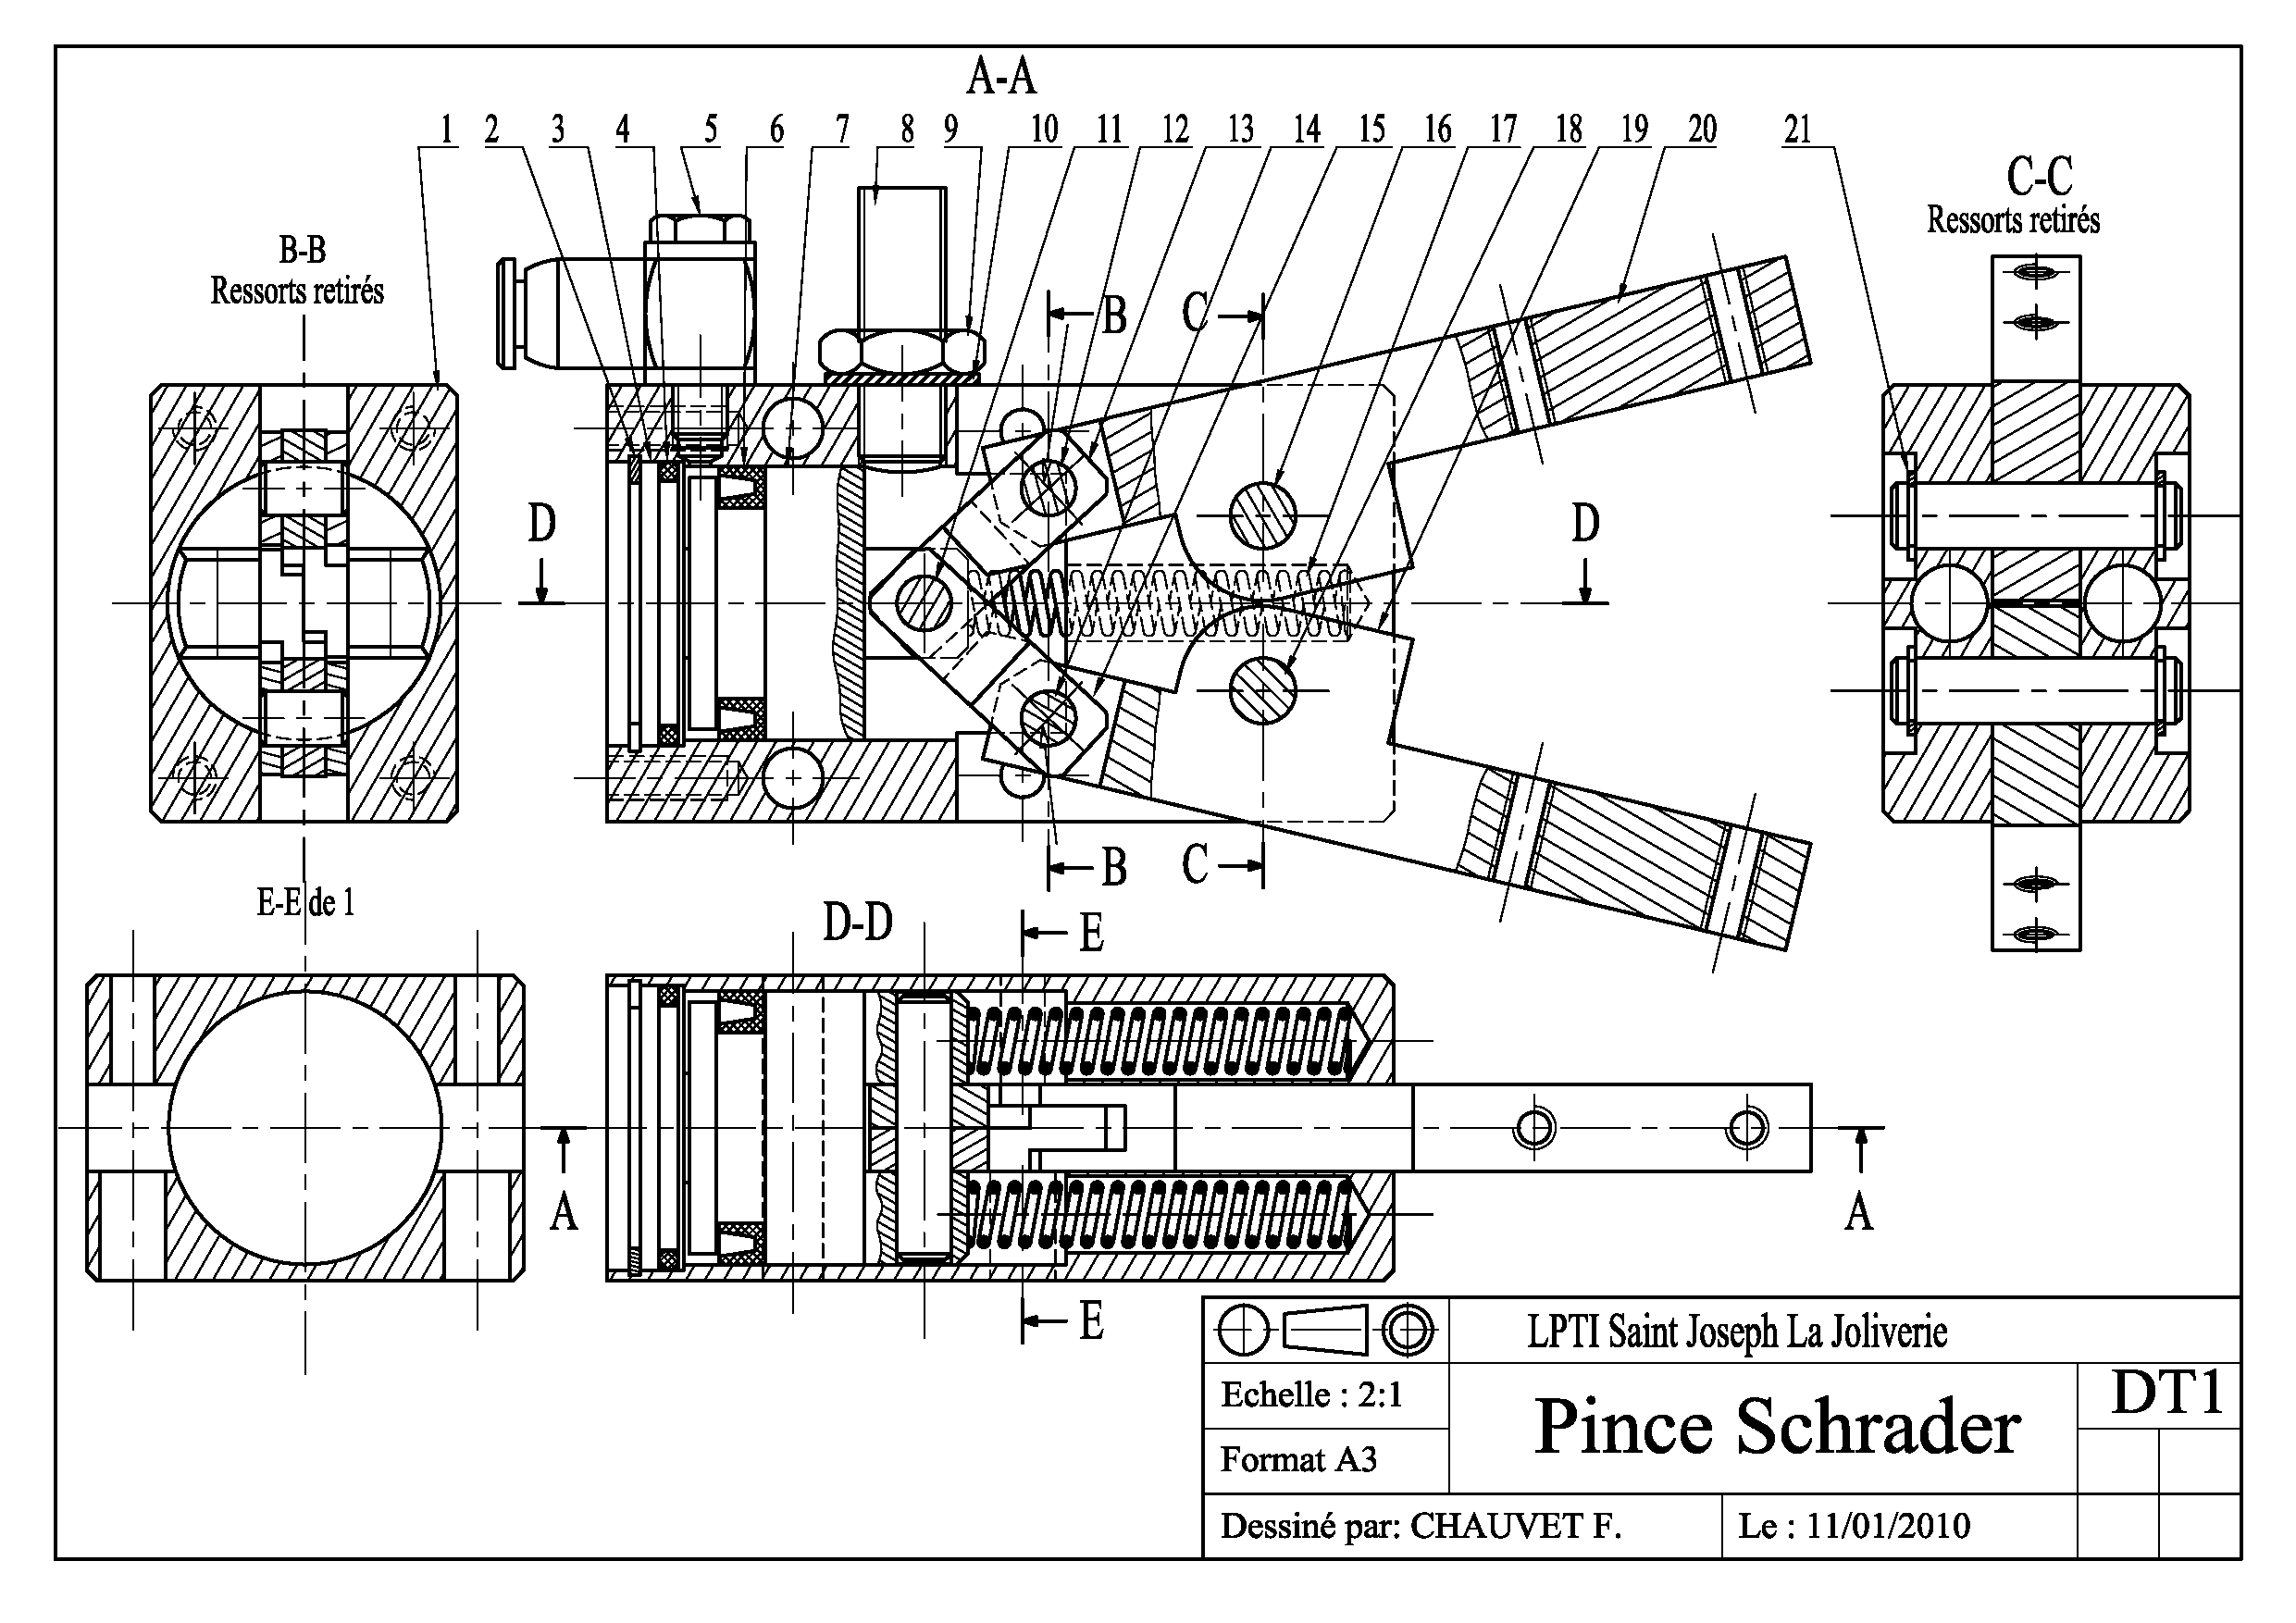
\includepdf[pages=-,nup=1x2]{pdf/dessin1.pdf}

%--------------------------------------------
\subsection{Dessin 2 -- Surfaceuse pneumatique}
\textbf{Il vous est demandé d'analyser le dessin industriel qui vous est présenté ci-desous avec le plus de précision possible.}\\
Cet exercice d'analyse consiste à mobiliser l'intégralité des connaissances de sciences industrielles, voir ceux d'autres cours.\\
Il est important d'avoir un raisonnement et une démarche clair. Je vous insite donc à suivre le modèle suivant :

\begin{enumerate}
\item Présenter la fonction principale du système étudié.
\item Décrire son fonctionnement.
\item Relever les originalités de conception du système sur le dessin.
\item Si possible, présenter les solutions techniques retenues par le concepteur (par exemple: pour étanchéifier le système).
\item Déterminer les moyens d'obtention des pièces principales présentées sur le dessin.
\end{enumerate}

\underline{Nota :} L'utilisation de diagrammes, croquis, et autres outils permettant de simplifier la compréhention de vos explexications sera être valorisée.

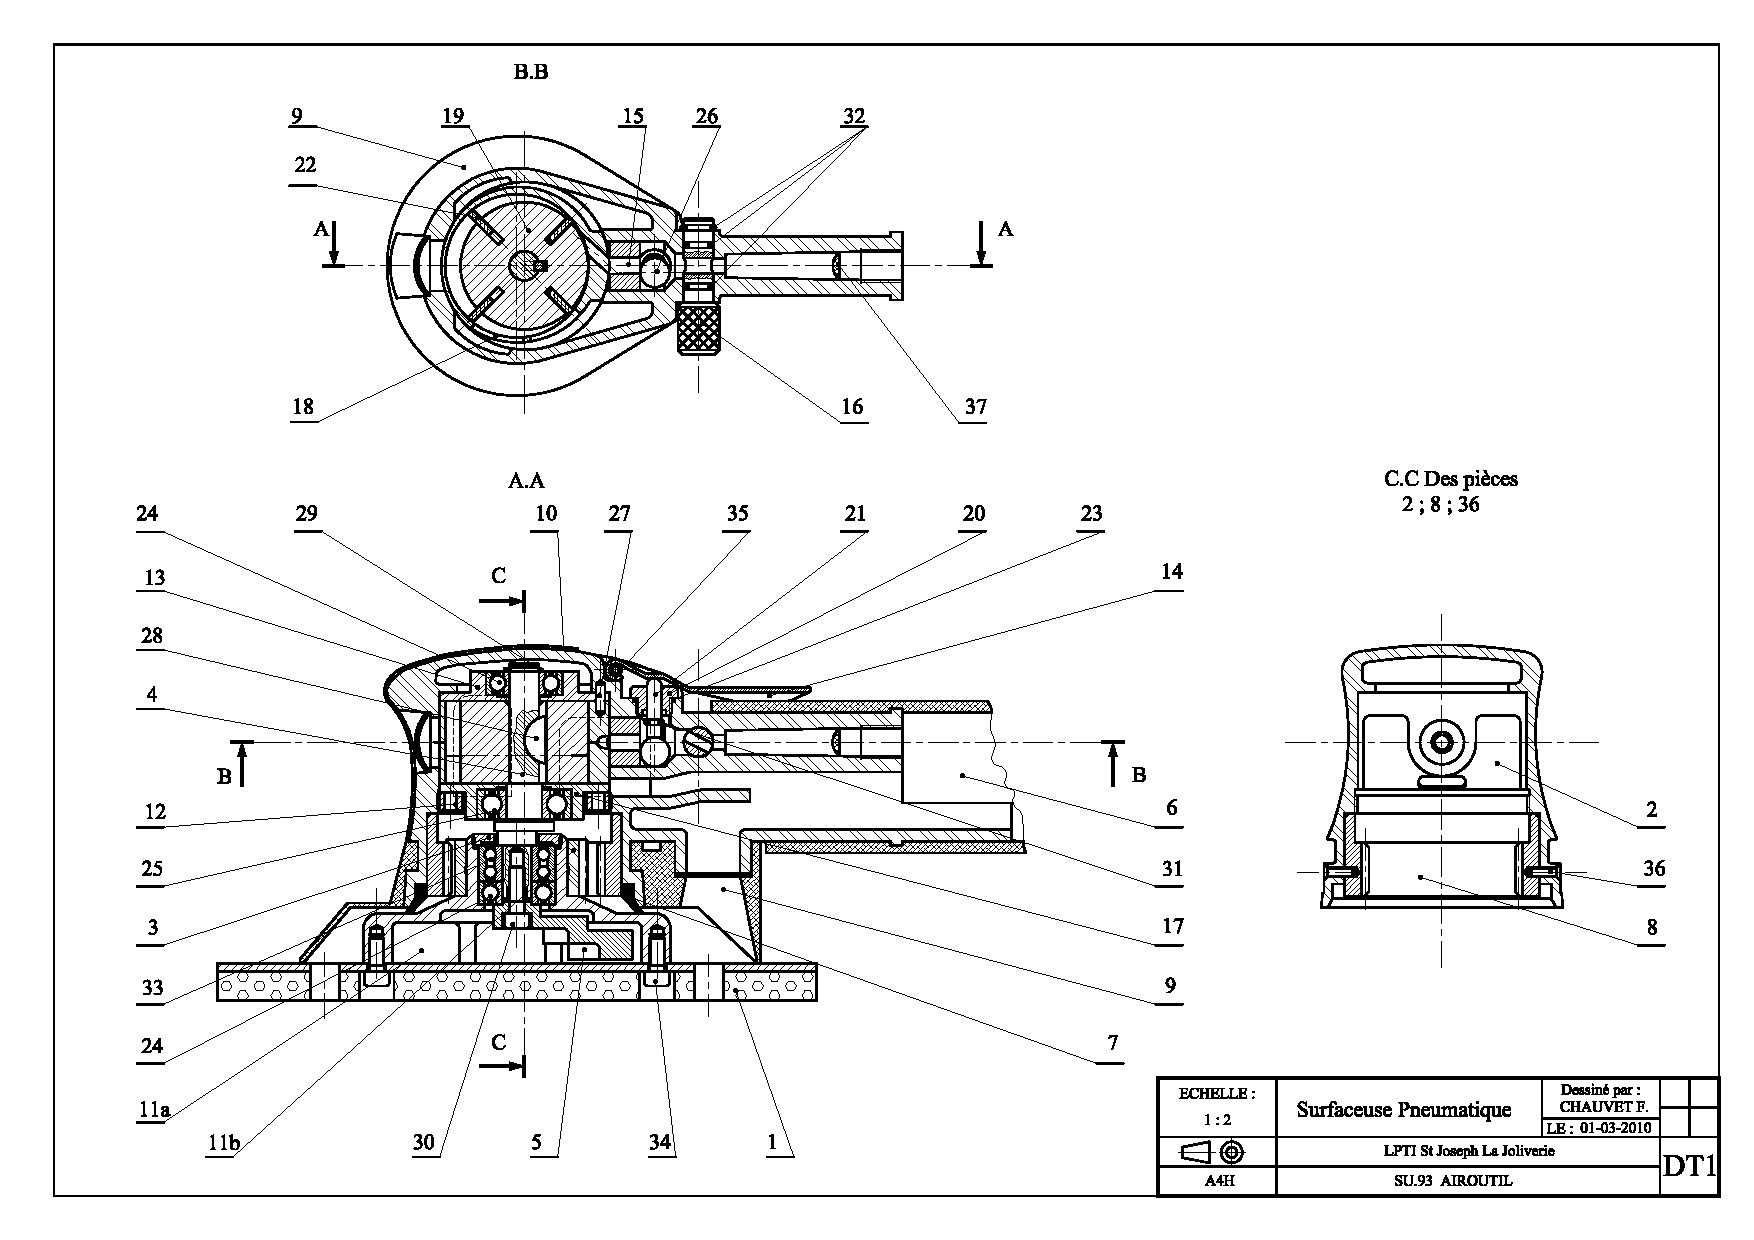
\includepdf[pages=-,nup=1x2]{pdf/dessin2.pdf}

%--------------------------------------------
\subsection{Dessin 3 -- Pompe doseuse}
\textbf{Il vous est demandé d'analyser le dessin industriel qui vous est présenté ci-desous avec le plus de précision possible.}\\
Cet exercice d'analyse consiste à mobiliser l'intégralité des connaissances de sciences industrielles, voir ceux d'autres cours.\\
Il est important d'avoir un raisonnement et une démarche clair. Je vous insite donc à suivre le modèle suivant :

\begin{enumerate}
\item Présenter la fonction principale du système étudié.
\item Décrire son fonctionnement.
\item Relever les originalités de conception du système sur le dessin.
\item Si possible, présenter les solutions techniques retenues par le concepteur (par exemple: pour étanchéifier le système).
\item Déterminer les moyens d'obtention des pièces principales présentées sur le dessin.
\end{enumerate}

\underline{Nota :} L'utilisation de diagrammes, croquis, et autres outils permettant de simplifier la compréhention de vos explexications sera être valorisée.

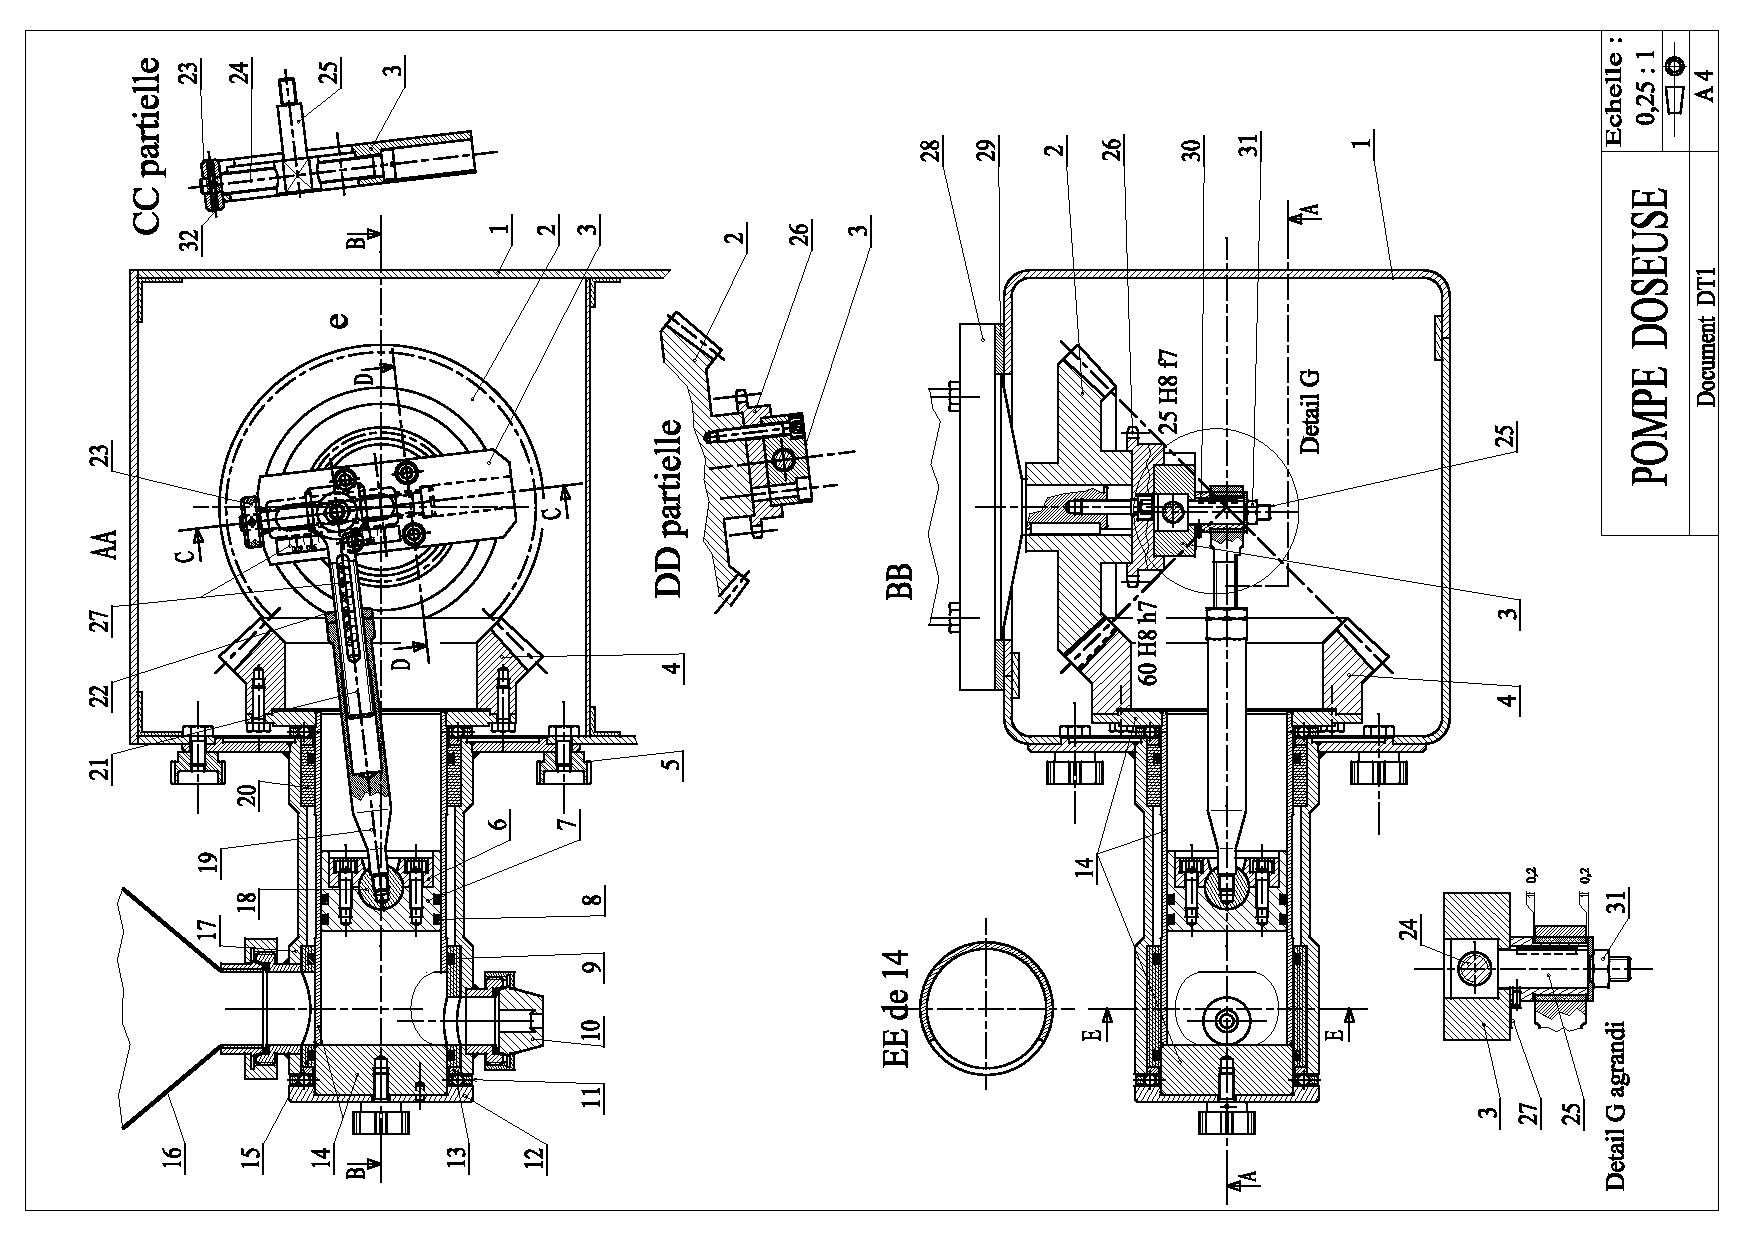
\includepdf[pages=-,nup=1x2]{pdf/dessin3.pdf}

%--------------------------------------------
\subsection{Dessin 4 -- Moteur Poclain}
\textbf{Il vous est demandé d'analyser le dessin industriel qui vous est présenté ci-desous avec le plus de précision possible.}\\
Cet exercice d'analyse consiste à mobiliser l'intégralité des connaissances de sciences industrielles, voir ceux d'autres cours.\\
Il est important d'avoir un raisonnement et une démarche clair. Je vous insite donc à suivre le modèle suivant :

\begin{enumerate}
\item Présenter la fonction principale du système étudié.
\item Décrire son fonctionnement.
\item Relever les originalités de conception du système sur le dessin.
\item Si possible, présenter les solutions techniques retenues par le concepteur (par exemple: pour étanchéifier le système).
\item Déterminer les moyens d'obtention des pièces principales présentées sur le dessin.
\end{enumerate}

\underline{Nota :} L'utilisation de diagrammes, croquis, et autres outils permettant de simplifier la compréhention de vos explexications sera être valorisée.

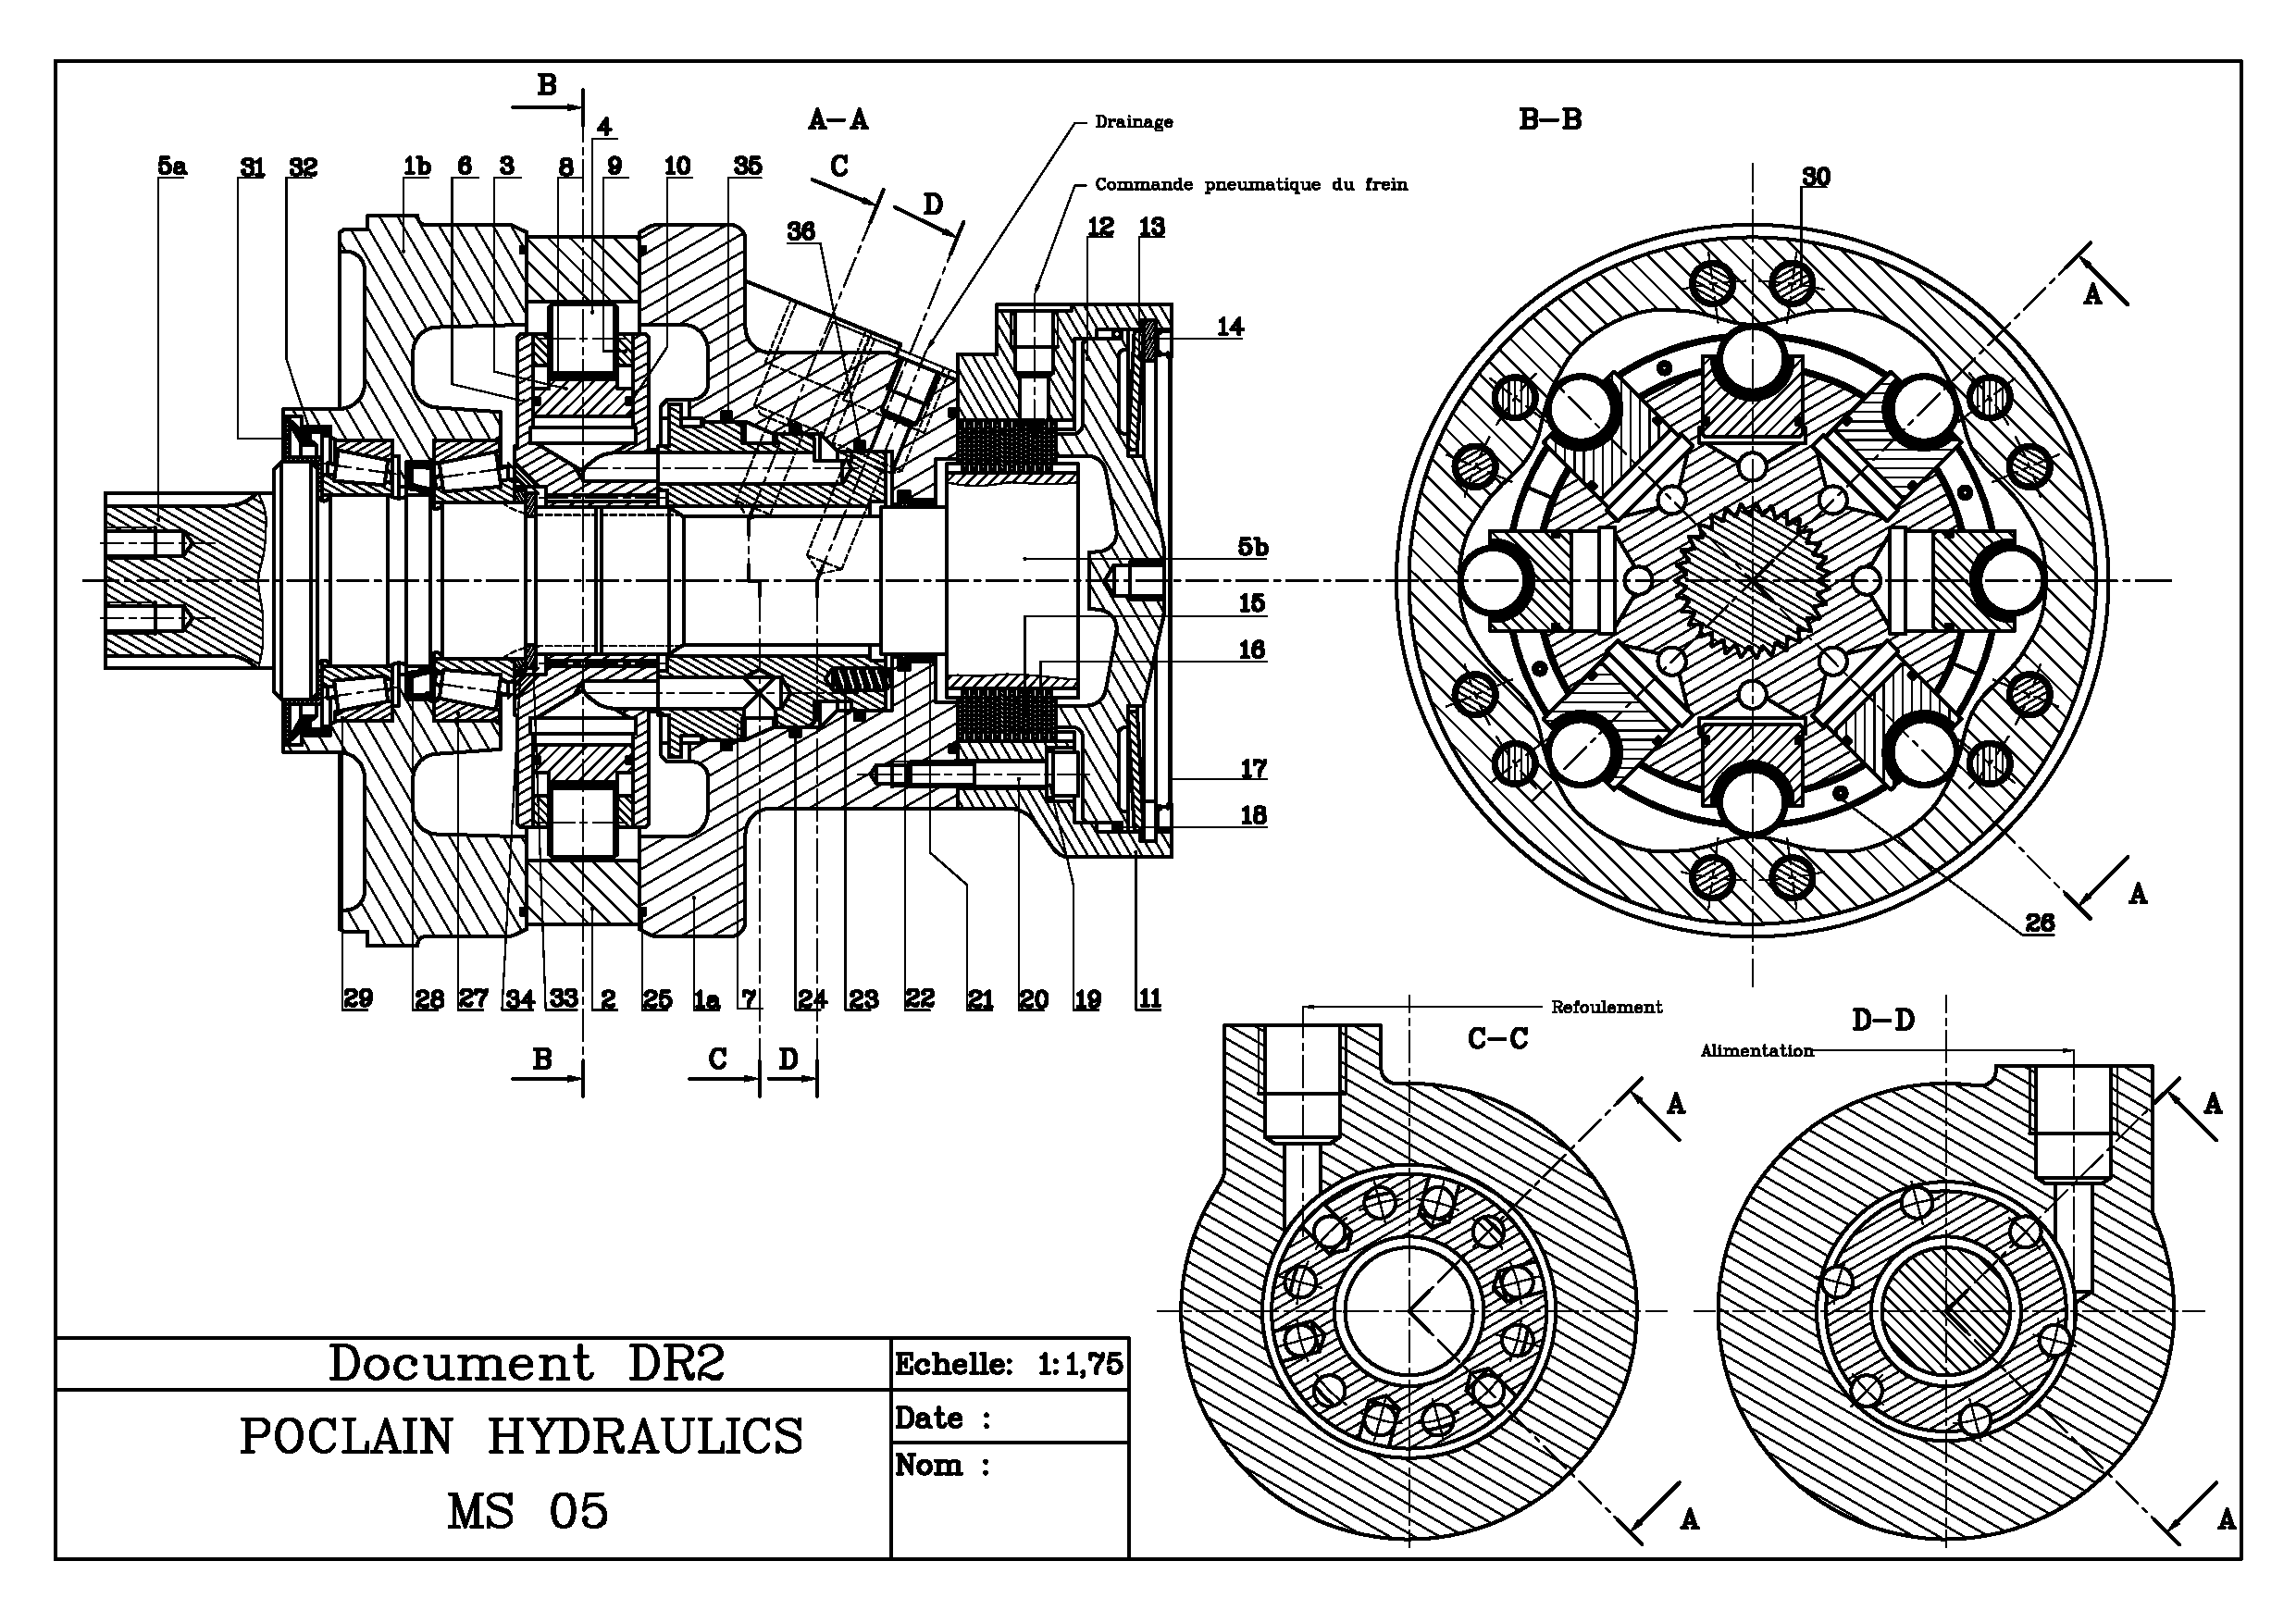
\includepdf[pages=-,nup=1x2]{pdf/dessin4.pdf}

%--------------------------------------------
\subsection{Dessin 5 -- Marteau perforateur}
\textbf{Il vous est demandé d'analyser le dessin industriel qui vous est présenté ci-desous avec le plus de précision possible.}\\
Cet exercice d'analyse consiste à mobiliser l'intégralité des connaissances de sciences industrielles, voir ceux d'autres cours.\\
Il est important d'avoir un raisonnement et une démarche clair. Je vous insite donc à suivre le modèle suivant :

\begin{enumerate}
\item Présenter la fonction principale du système étudié.
\item Décrire son fonctionnement.
\item Relever les originalités de conception du système sur le dessin.
\item Si possible, présenter les solutions techniques retenues par le concepteur (par exemple: pour étanchéifier le système).
\item Déterminer les moyens d'obtention des pièces principales présentées sur le dessin.
\end{enumerate}

\underline{Nota :} L'utilisation de diagrammes, croquis, et autres outils permettant de simplifier la compréhention de vos explexications sera être valorisée.

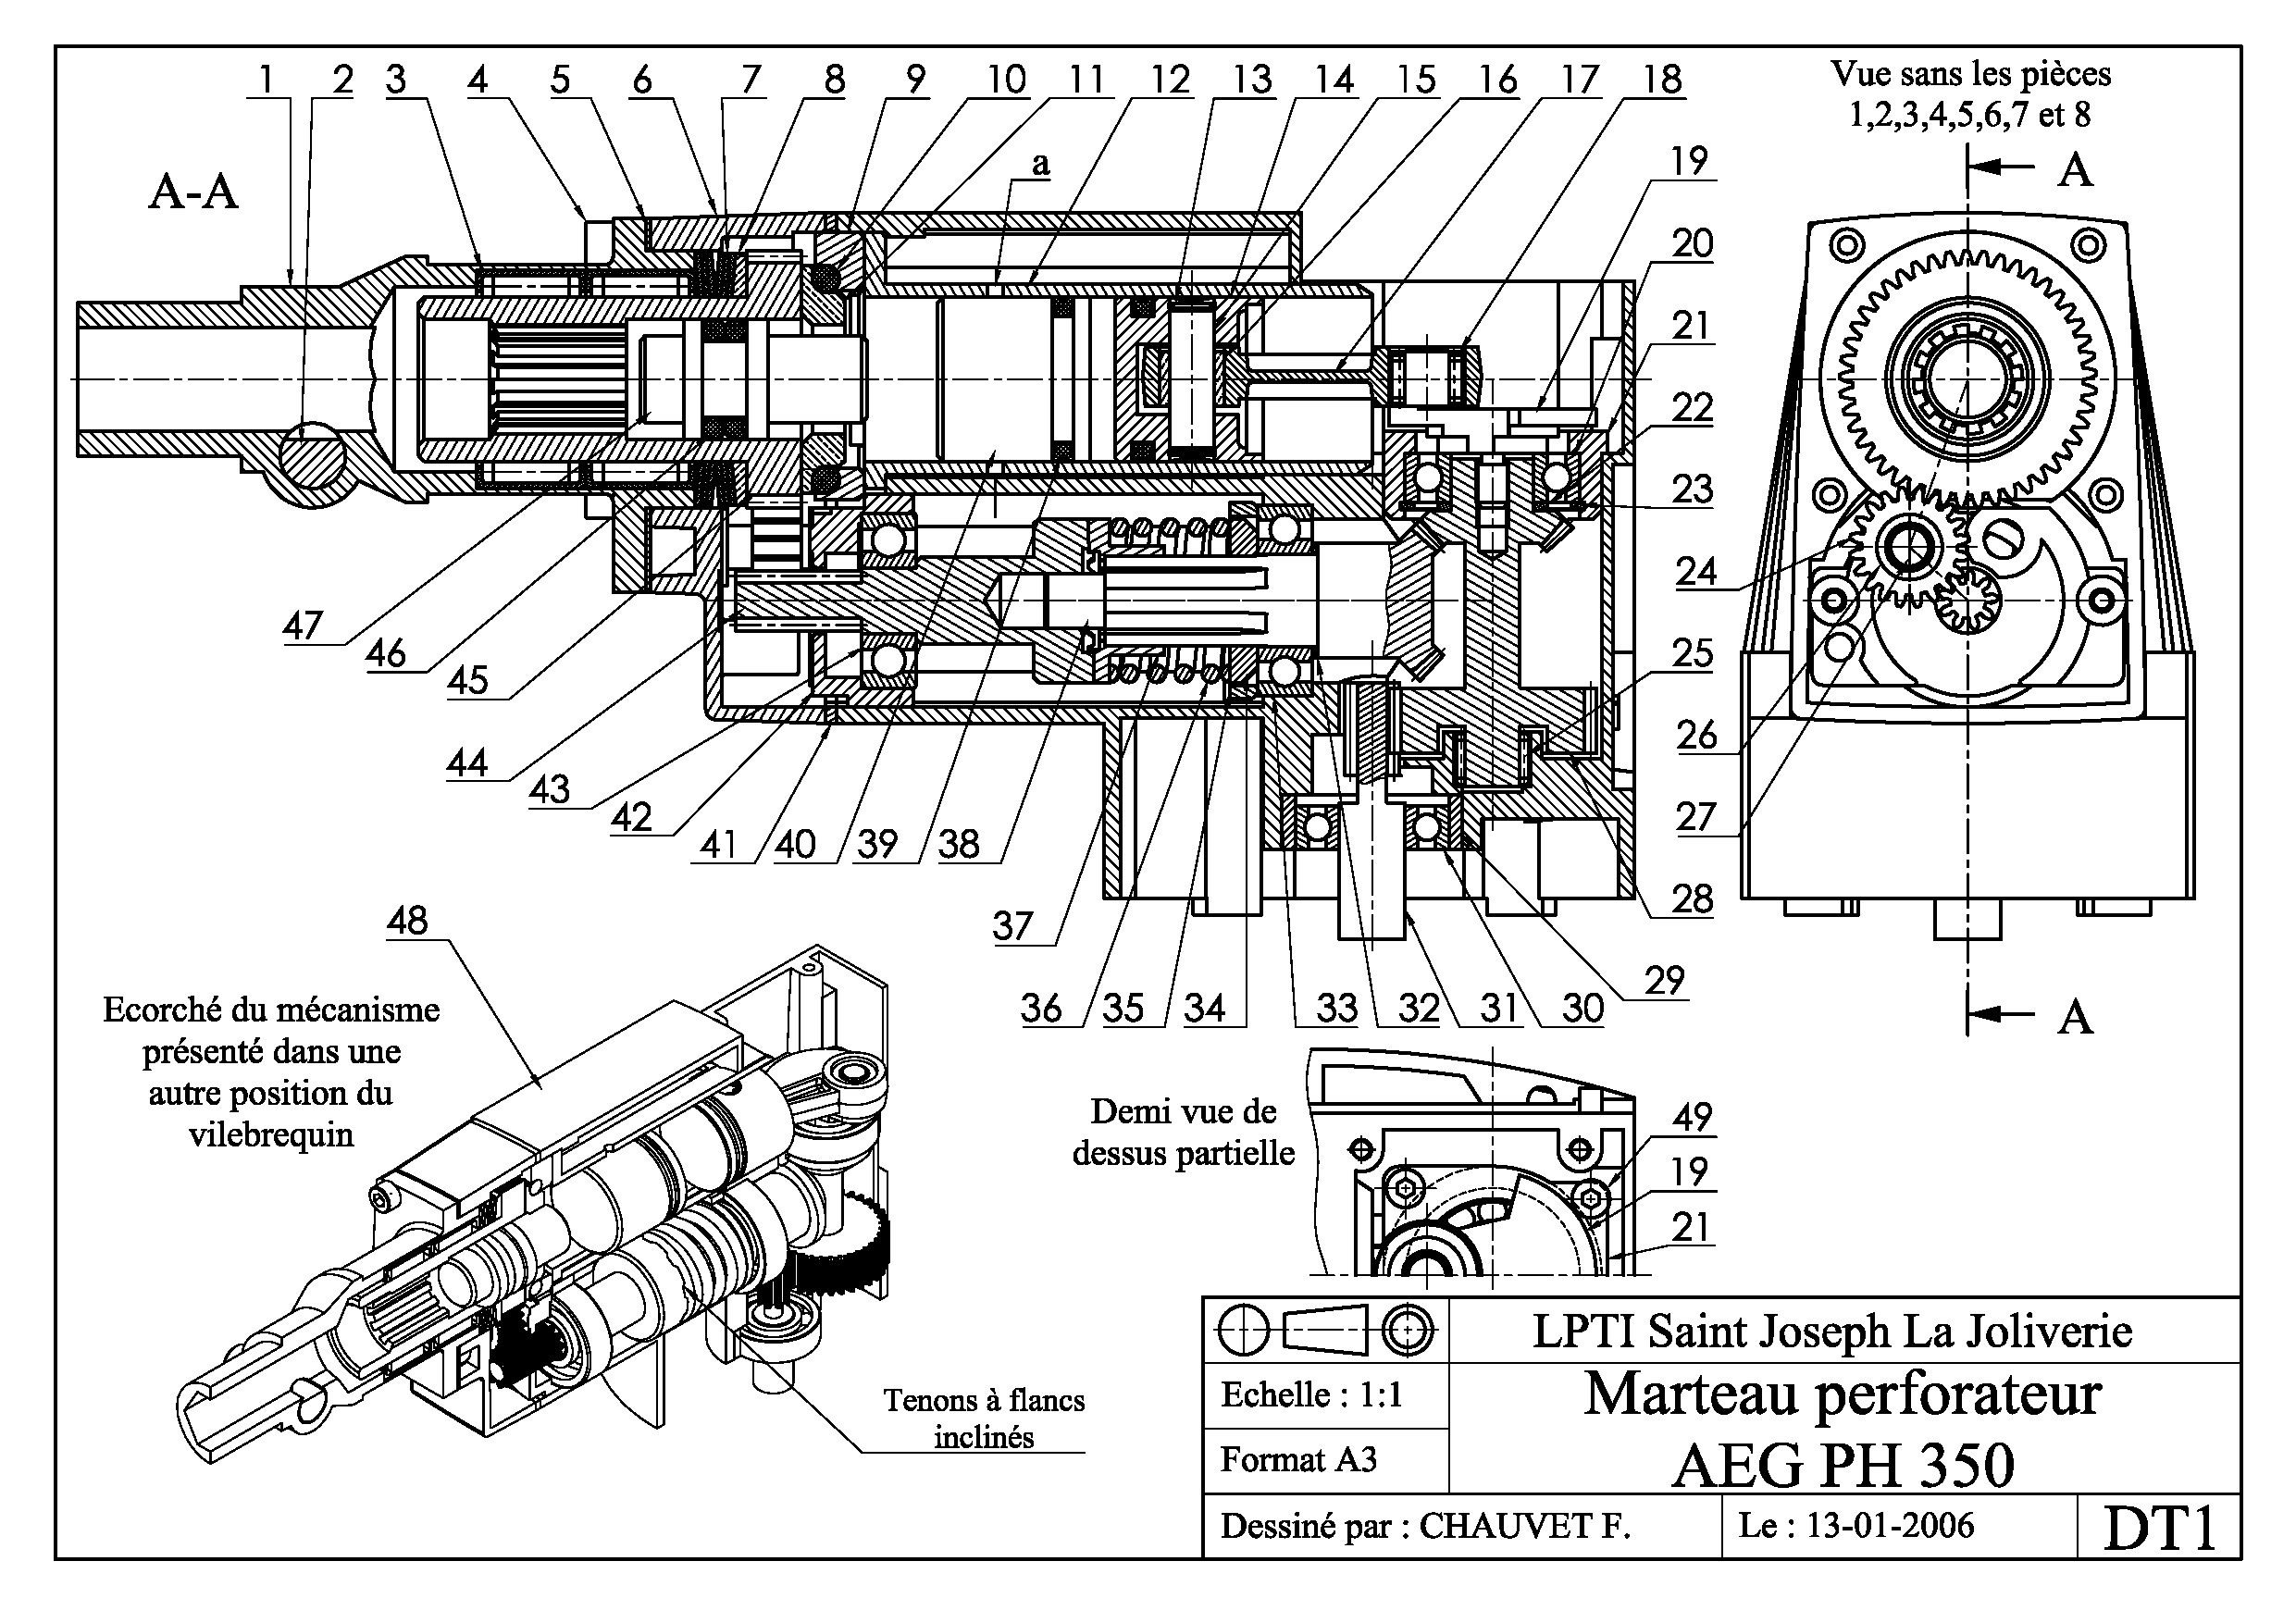
\includepdf[pages=-,nup=1x2]{pdf/dessin5.pdf}

%--------------------------------------------
\subsection{Dessin 6 -- Mesureur volumétrique}
\textbf{Il vous est demandé d'analyser le dessin industriel qui vous est présenté ci-desous avec le plus de précision possible.}\\
Cet exercice d'analyse consiste à mobiliser l'intégralité des connaissances de sciences industrielles, voir ceux d'autres cours.\\
Il est important d'avoir un raisonnement et une démarche clair. Je vous insite donc à suivre le modèle suivant :

\begin{enumerate}
\item Présenter la fonction principale du système étudié.
\item Décrire son fonctionnement.
\item Relever les originalités de conception du système sur le dessin.
\item Si possible, présenter les solutions techniques retenues par le concepteur (par exemple: pour étanchéifier le système).
\item Déterminer les moyens d'obtention des pièces principales présentées sur le dessin.
\end{enumerate}

\underline{Nota :} L'utilisation de diagrammes, croquis, et autres outils permettant de simplifier la compréhention de vos explexications sera être valorisée.

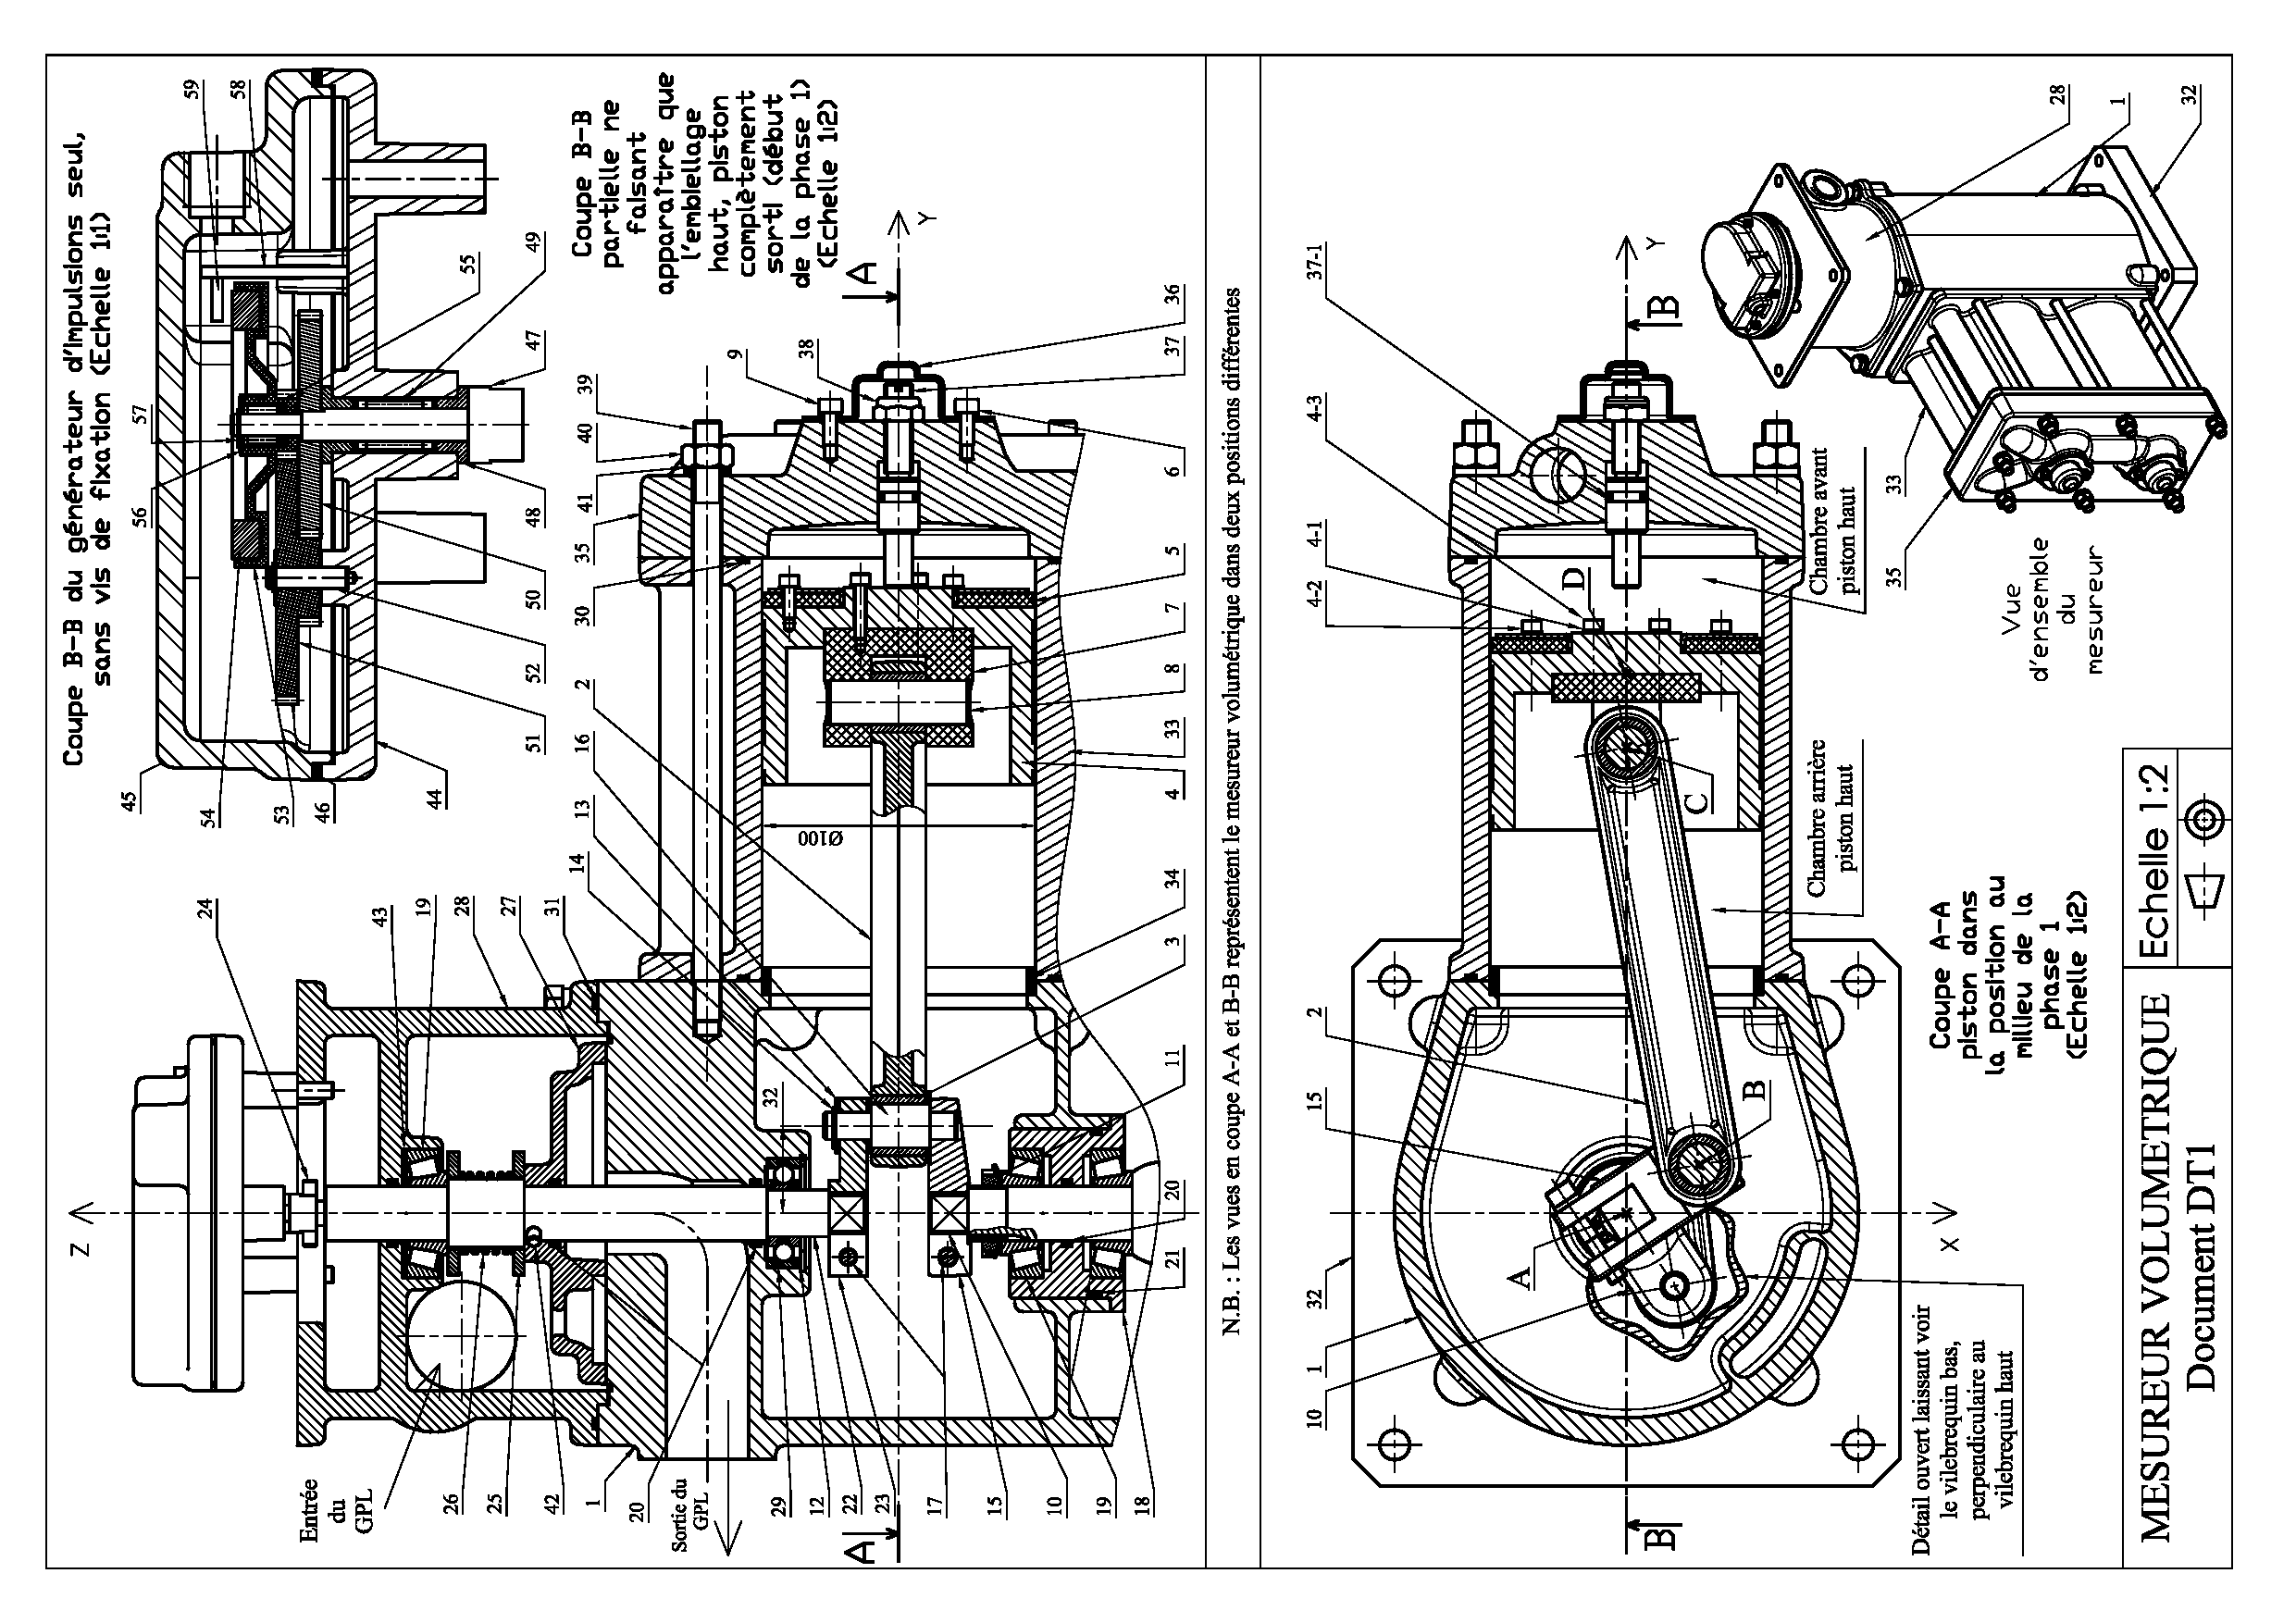
\includepdf[pages=-,nup=1x2]{pdf/dessin6.pdf}

%----------------------------------------------------------------------------------------
%	Seconde série
%----------------------------------------------------------------------------------------

\section{Seconde série}

La seconde série de dessins industriels se trouve à l'adresse suivante :

\vspace*{\baselineskip}
\begin{center}
\texttt{\url{http://perso.crans.org/oleveque/CPGE/dessins_industriels}}
\end{center}

